\documentclass[14pt]{article}
\usepackage{xcolor}
\usepackage{graphicx}
\usepackage{enumitem}
\setlist[enumerate]{label*=\arabic*.}
\usepackage{url}
\usepackage{setspace}
\usepackage[italian]{babel}
\usepackage[T1]{fontenc}
\usepackage[a4paper,top=1.2cm,bottom=2.2cm,left=2cm,right=2cm]{geometry}
\usepackage{multicol}
\usepackage{hhline}
\usepackage{amstext}
\usepackage{amsmath}
\usepackage{amssymb}
\usepackage{pifont}
\usepackage{subfigure}
\usepackage{hhline}
\usepackage{multirow}
\title{ Sample size and z test for two independent \\Bernoulli samples with the same size}
\author{}
\date{}

\begin{document}
\maketitle

\section{Introduction: things to keep in mind about ...}
\subsection{Bernoulli random variables and normal approximation of the sample mean}\label{bernoulli}
Given $X_{1},\dots,X_{n_{1}}$ a random sample of size $n_{1}$ drawn from a Bernoulli population $X$ of parameter $p_{1}$ and $Y_{1},\dots,Y_{n_{2}}$ a random sample of size $n_{2}$ drawn from a Bernoulli population $Y$ of parameter $p_{2}$ independent of  $X$, we are interested in studying the relationship between sample size and effect siz e $\left | p_{1}-p_{2}\right |$ in comparing the sample mean $\overline{X}_{(n_{1})}=\frac{1}{n_{1}} \sum_{i=1}^{n_{1}} X_i$ and $\overline{Y}_{(n_{2})}=\frac{1}{n_{2}} \sum_{i=1}^{n_{2}}Y_i$ at a given significance level $\alpha$ and, in a second step, with a given power $1-\beta$. 
For our purposes we use samples of the same size, namely $n_{1}=n_{2}=n$ so we can refer to the sample means simply as: $\overline{X}$ and $\overline{Y}$.\\
\textit{Remark: }in general the effect size for comparing two means is given by $\frac{\left |\mu_{0}-\mu_{1}\right |}{\sigma}$; as it will be clear soon, here, since we use an upper bound for the standard deviation of a Bernoulli distribution, we can neglect ${\sigma}$.\\
\newline
The expected value and the variance of a Bernoulli random variable of parameter $p$ are respectively  $p$ and $p\cdot(1-p)$. It is also  easy to show that the variance is bounded above by $0.25$, ad the maximum is reached at $p=1/2$.
 Therefore  $E(X)=p_{1}$, $var(X)= p_{1}\cdot(1-p_{1})\leq1/4$ and $E(Y)=p_{2}$, $var(Y)= p_{2}\cdot(1-p_{2})\leq1/4$. \\
Being the sample mean an unbiased estimator for the expected value, it holds that $E(\overline{X}=p_{1})$ and $E(\overline{Y}=p_{2})$.\\
\newline
Let $D=\overline{X}-\overline{Y}$.\\
It holds that: $E(D)=p_{1}-p_{2}$ and, since $X\perp Y$, it also holds that: \\
 $var(D)=var \left (\overline{X}-\overline{Y}\right )=\frac{var \left (\sum_{i=1}^{n_{1}} X_i \right )+var\left(\sum_{i=1}^{n_{1}} Y_i \right )}{n^2}=\frac{p_{1}\cdot(1-p_{1})+p_{2}\cdot(1-p_{2})}{n}$, that implies\\
 \begin{equation}
\sigma_{D}=\sqrt{\frac{p_{1}\cdot(1-p_{1})+p_{2}\cdot(1-p_{2})}{n}}\leq \sqrt{\frac{1}{2\cdot n}}
\end{equation}
\newline
\newline
Let $D^{*}$  the standardization of $D$, namely \\ 
\begin{equation}
D^{*}=\frac{D-E(D)}{\sqrt{var(D)}}=\frac{(\overline{X}-\overline{Y})-(p_{1}-p_{2})}{\sqrt{\frac{p_{1}\cdot(1-p_{1})+p_{2}\cdot(1-p_{2})}{n}}}
\end{equation}
\newline
The sum of $n$ independent and identically distributed Bernoulli random variables with  parameter  $p$ follows a binomial distribution whose parameters are $n$ and $p$.
If we suppose $n\gg1$, the binomial distribution can be approximated by a Normal distribution, and the approximation is already good starting from values of $n$ on the order of magnitude of $10^{2}$.  In this approximation it holds that  $D$ follows a Normal distribution and $D^{*}\sim N(0,1)$, so it is possible to compute a sufficient sample size starting from the Normal random variable. \textit{Remark: } This observation is important because, in order to apply the Central Limit Theorem, 
$n$ must tend to infinity; if the theorem is used to find the value of $n$, it is necessary to verify whether for the original distribution (in our case a Bernoulli distribution) that value is large enough to allow a good approximation of the sample mean with a normal distribution.\\

\subsection{standard Normal variables}
The cumulative distribution function of a standard Normal variable $D^{*}$ is called $\Phi$, that is $\Phi (x)=P(D^{*}\leq x)$.\\
\newline
As the standard Normal distribution is an even function, called $z_{\alpha}$ the $\alpha$-quantile of the distribution, it holds that  \\
\begin{equation}\label{eq: zalfa}
z_{\alpha}=-z_{1-\alpha} \text{, and, equivalently: } \left |z_{\alpha}\right |=\left |z_{1-\alpha} \right |
\end{equation}\\
\textit{Remark: } sometimes in the literature $z_{\alpha} $ is referred to as the upper quantile 
$\alpha$ and is such that $P(D^{*}\geq z_{\alpha}).$\\
It is  easy to show that 
\begin{equation}\label{eq: 2 fi minus 1}
P \left ( \left | D^{*} \right| \leq k \right )=2\cdot \Phi (k) -1
\end{equation}\\
Since a linear function of a Normal random variable is still a Normal random variable, it  holds that
\begin{equation}
D\sim N\left (E(D),\sqrt{var(D)} \right )
\end{equation}

\subsection{hypothesis testing}

Consider the \textbf{null hypothesis} $H_{0}: p_{1}=p_{2}=p$ vs. $H_{1}: p_{1}\neq p_{2}$. \\
\newline
We commit a \textbf{type I error} if we reject $H_{0}$ when  $H_{0}$ is true.\\
\newline
The \textbf{significance level $\alpha$} of the test is the probability of committing a type I error, that is $\alpha=P_{H_{0}} \left (\text{reject } H_{0} \right)$.\\
\newline
Given a statistic $T_{n}$, a \textbf {critical region $C$} at significance level $\alpha$ is the region of rejection of $H_{0}$, that is $C$ is such that  $P_{H_{0}}(T_{n}\in C)=\alpha$.\\
\newline
We commit a \textbf{type II error} if we do not reject $H_{0}$ when  $H_{0}$ is false.\\
\newline
If we call $\beta$ the probability of  committing a type II error, that is 
$ \beta= P_{H_{1}}  \left ( \text{not reject } H_{0} \right )$, 
 the \textbf{power} of the test is the probability $1-\beta$ of rejecting $H_{0}$ when  $H_{0}$ is false, that is  $1-\beta=P_{H_{1}} \left (\text{reject } H_{0}\right)$. 
%\newline

% let's assume $\alpha < 0.5 $ without loss of generality, \textbf{we require that} $P_{H_{0}}(\left|{D}\right|>c)\leq\alpha$, which implies


\section{Sample size at a given significance level $\alpha$ for a two-sided test}
Consider the null hypothesis $H_{0}: p_{1}=p_{2}=p$ vs. $H_{1}: p_{1}\neq p_{2}$ at significance level $\alpha$ (assume $\alpha < 0.5 $ without loss of generality).
Requiring a \textbf{significance level $\alpha$} is equivalent to requiring
\begin{equation}\label{eq: critical region alfa}
P_{H_{0}}(\left | D>c \right |)\leq\alpha
\end{equation}
Let us call $c>0$ \textit{critical value}.\\
\newline
If \textbf{If $H_{0}$ is true}, then $E(D)=0$, and

\begin{equation}
\begin{split}
 \alpha\geq P_{H{0}} (\left | D \right |\geq c)=\\
 P_{H{0}} (\left | D \right |\geq c)= P(\left | D /\sigma_{D}\right |\geq c/\sigma_{D})=\\
P(\left | D^{*}\right |\geq c/\sigma_{D})=2-2\cdot\Phi(c/\sigma_{D})
  \end{split}
 \end{equation}\newline
 that implies 
 \begin{equation}\label{eq: critical region}
\Phi\left ( \frac{c}{\sigma_{D}}\right ) \geq1-\frac{\alpha}{2}
\end{equation}\newline
The minimum value $c/\sigma_{D}$ satisfying the equation in (\ref{eq: critical region}) is therefore the $(1-\alpha/2)$-quantile of the standard Normal distribution, and we \textbf{reject $H_{0}$} if $\left |D^{*} \right | \geq z_{1-\alpha/2}  $, that is if \\
%namely $c/\sigma_{D} =z_{1-\alpha/2}= \left |z_{\alpha/2} \right | $, which implies $c=\sigma_{D}\cdot z_{1-\alpha/2}$ 
\begin{equation}
\left |\frac{(\overline{X}-\overline{Y})}{\sqrt{\frac{2 \cdot p \cdot(1-p)}{n}}}\right | \geq  z_{1-\alpha/2} \end{equation}\newline
In order to turn $\left |\frac{(\overline{X}-\overline{Y})}{\sqrt{\frac{2 \cdot p \cdot(1-p)}{n}}}\right |$ into a statistic (getting rid of the unknown parameter $p$), note that
\begin{equation}
  \sigma_{D} \leq \sqrt{\frac{1}{2\cdot n}} \text{ implies } c/\sigma_{D}\geq \sqrt{2\cdot n}\cdot c
\end{equation}\newline
and that, being $\Phi$ is a  monotonic increasing function, it holds that 
\begin{equation}\Phi(c/\sigma_{D})\geq 1-\alpha/2 \text{ for } c/\sigma_{D}\geq z_{1-\alpha/2}\end{equation}
Therefore we can reason in the worst case 
\begin{equation}\label{eq: critical value chain}
\left | \frac{(\overline{X}-\overline{Y})}{\sqrt{\frac{2 \cdot p \cdot(1-p)}{n}}} \right | \geq \left | \frac{(\overline{X}-\overline{Y})}{\sqrt{\frac{1}{2 \cdot n}}} \right | \geq z_{1-\alpha/2}
\end{equation}
\newline
%Now it is possible to calculate the sufficient sample size $n$ that assures  $P_{H_{0}}(|D|>c)\leq\alpha$ by solving~(\ref{eq: critical value chain})  with respect to $n$, obtaining \\
Solving with respect to $n$ we obtain:
\begin{equation}
n \geq \frac{1}{2}\cdot \left ( \frac{z_{1-\alpha/2}}{\overline{X}-\overline{Y}}  \right )^{2}
\end{equation}
\newline
If we want to be able to detect a significant difference at least equal to $d$ (effect size) at level $\alpha$ it is therefore sufficient that
 \begin{equation}
\textcolor{red}{n \geq} \frac{1}{2}\cdot \left ( \frac{z_{1-\alpha/2}}{\overline{X}-\overline{Y}}  \right )^{2} \geq\textcolor{red}{\frac{1}{2}\cdot \left ( \frac{z_{1-\alpha/2}}{d}  \right )^{2}}
\end{equation}
\newline
It is worth to note that $n$ is inversely proportional to the square of the effect size. \\
Fig.~\ref{fig:sample size alpha} shows the sufficient sample size $n$ as a function of effect size at different significance levels $\alpha$.


\begin{figure}[h!]
\centering
\begin{minipage}{0.31\textwidth}
  \centering
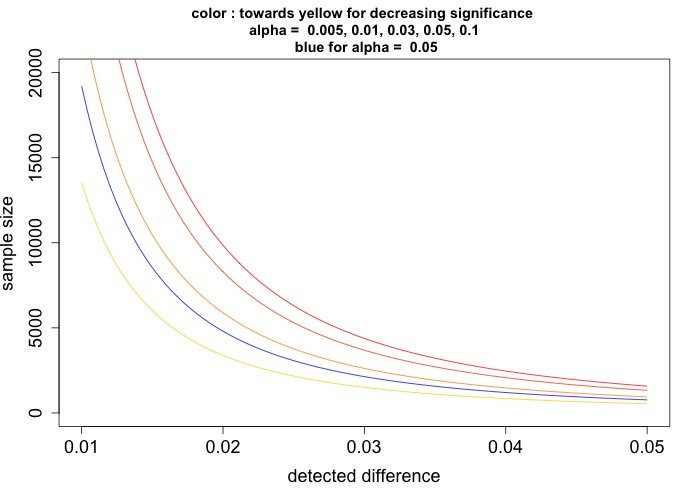
\includegraphics[scale=0.23]{plots/plot_samplesize VS effectsize_alfa 1.jpg}  
\end{minipage}
\begin{minipage}{0.31\textwidth}
  \centering
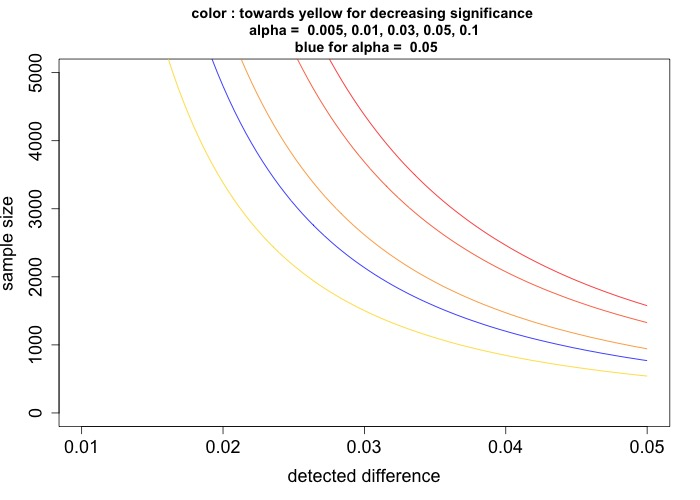
\includegraphics[scale=0.23]{plots/plot_samplesize VS effectsize_alfa 2.jpg}  
\end{minipage}
\begin{minipage}{0.31\textwidth}
  \centering
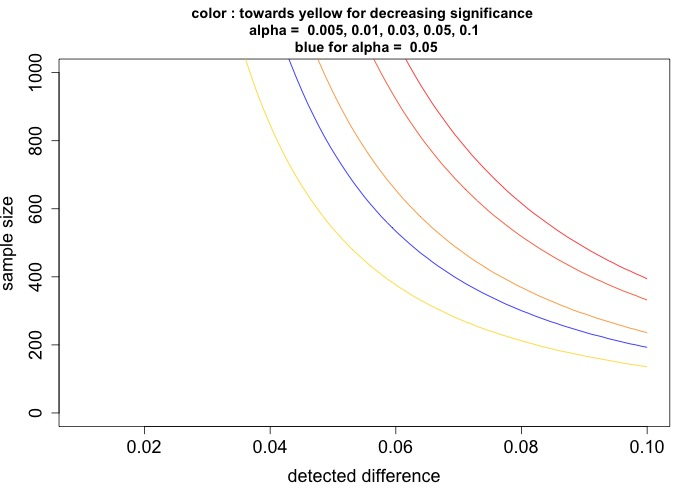
\includegraphics[scale=0.23]{plots/plot_samplesize VS effectsize_alfa 3.jpg}  
\end{minipage}
\caption{$n$ as a function of effect size}
\label{fig:sample size alpha}
\end{figure}

\section{Sample size at a given significance level $\alpha$ and power $1-\beta$ for a two-sided test}
Now we take int account also type II error: not reject $H_{0}$ when it is false, whose probability is $\beta$. \\\textbf{If $H_{1}$ is true}, we have to explicitly take into account the two means $p_{1}$ and $p_{2}$, since $E(D)=p_{1}- p_{2}$. So let's restart from the very beginning. First of all recall that (type I error):
\begin{equation}
\begin{split}
 \alpha\geq P_{H{0}} (\left | D \right |\geq c)=1-\left (2\cdot\Phi\left ( \frac{c}{\sigma_{D}}\right ) -1\right ) \text{ that implies }\\
\Phi\left ( \frac{c}{\sigma_{D}}\right ) =1-\frac{\alpha}{2}\text{ and the critical values }
c_{1}=z_{1-\frac{\alpha}{2}}\cdot\sigma_{D} \text{ and } c_{2}=-z_{1-\frac{\alpha}{2}}\cdot\sigma_{D}= z_{\frac{\alpha}{2}}\cdot\sigma_{D}.
\end{split}\end{equation}\newline
Then we require that (type II error): $P_{H{1}} (\left | D \right |\leq c) \leq \beta$ , or, equivalently, that $ P_{H{1}} (\left | D \right |\geq c) \geq 1-\beta$, that is
\begin{equation}
 \begin{split}
1-\beta\leq P_{H{1}} (\left | D \right |\geq c) = P_{H{1}} (\left | D \right |\geq  z_{1-\frac{\alpha}{2}}\cdot\sigma_{D}) = \\
P_{H{1}} \left (D>  z_{1-\frac{\alpha}{2}}\cdot\sigma_{D} \cup D\leq  z_{\frac{\alpha}{2}}\cdot\sigma_{D} \right ) = 
P_{H{1}} \left (D>  z_{1-\frac{\alpha}{2}}\cdot\sigma_{D}\right )  + P_{H{1}} \left (D\leq  z_{\frac{\alpha}{2}}\cdot\sigma_{D}\right ) =\\
P\left (\frac{D-(p_{1}- p_{2})}{\sigma_{D} } >z_{1-\frac{\alpha}{2}} - \frac{(p_{1}- p_{2})}{\sigma_{D}} \right )+
P\left (\frac{D-(p_{1}- p_{2})}{\sigma_{D} } \leq z_{\frac{\alpha}{2}}-\frac{(p_{1}- p_{2})}{\sigma_{D}} \right )=\\
P\left (D^{*}>z_{1-\frac{\alpha}{2}}-\frac{(p_{1}- p_{2})}{\sigma_{D}} \right )+
P\left (D^{*} \leq z_{\frac{\alpha}{2}}-\frac{(p_{1}- p_{2})}{\sigma_{D}}   \right )=\\
1-\Phi\left (z_{1-\frac{\alpha}{2}}- \frac{(p_{1}- p_{2})}{\sigma_{D}} \right )+\Phi\left ( z_{\frac{\alpha}{2}}-\frac{(p_{1}- p_{2})}{\sigma_{D}} \right )
 \end{split}
\end{equation}
Taking the upper bound $\sqrt{\frac{1}{2\cdot n}}$ for $\sigma_{D}$, the plot of $1-\beta$ against $(p_{1}- p_{2})$ for different significance levels and in the particular case of $n=100$ is shown in Figure \ref{fig:power}, while in Figure \ref{fig:power n} the power function is plot for different sample sizes in the particular case of $\alpha=0.05$.
\newline
Note that  $1-\beta$ is an even function, see the plot it against $\left  |p_{1}- p_{2} \right |$ . Therefore we can consider the case $( p_{1}- p_{2} ) >0 $. It holds that $\Phi\left ( z_{\frac{\alpha}{2}}-\frac{(p_{1}- p_{2})}{\sigma_{D}} \right )< \alpha/2$, and we can neglect it, getting
\begin{equation}
\beta \lessapprox \Phi \left (z_{1-\frac{\alpha}{2}}- \frac{(p_{1}- p_{2})}{\sigma_{D}} \right )
\end{equation}
Therefore
\begin{equation}
z_{\beta}\simeq z_{1-\frac{\alpha}{2}} - (p_{1}- p_{2})/\sigma_{D} \text{ and, for (\ref{eq: zalfa})  it holds that: } -z_{1-\beta} \simeq z_{1-\frac{\alpha}{2}}- (p_{1}- p_{2})/\sigma_{D}
\end{equation}\newline
%and, for (\ref{eq: zalfa})  it holds that: $-z_{1-\beta}=z_{1-\frac{\alpha}{2}}- (p_{1}- p_{2})/\sigma_{D}$\\
%\newline
\begin{figure}[h!]
\centering
\begin{minipage}{0.4\textwidth}
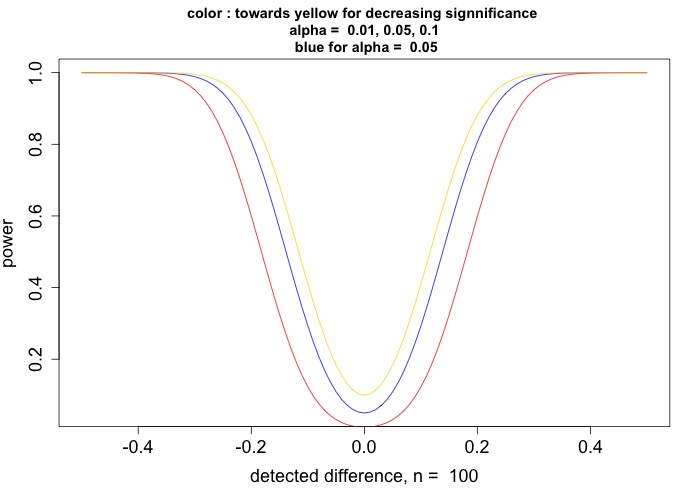
\includegraphics[scale=0.2]{plots/plot_power colore alfa 1.jpg}  
\end{minipage}
\begin{minipage}{0.4\textwidth}
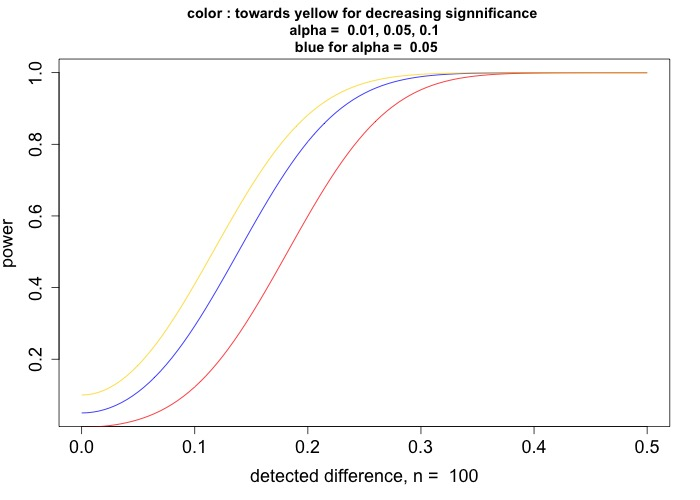
\includegraphics[scale=0.2]{plots/plot_power colore alfa 2.jpg}  
\end{minipage}
\caption{power as a function of effect size for different significance levels}
\label{fig:power}
\end{figure}

\begin{figure}[h!]
\centering
\begin{minipage}{0.4\textwidth}
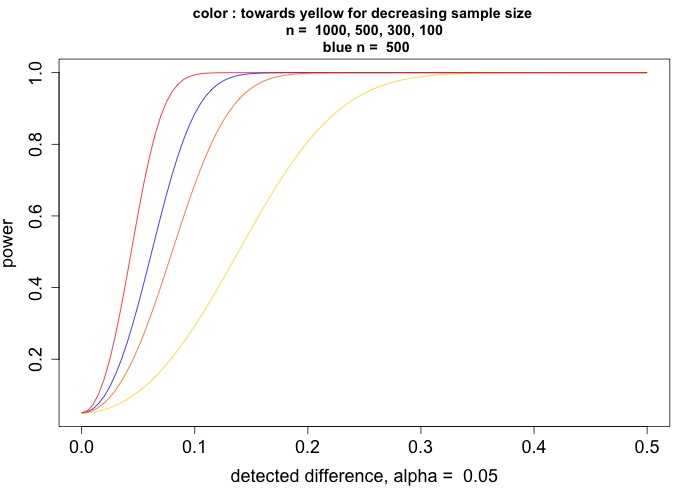
\includegraphics[scale=0.2]{plots/plot_power colore size 1.jpg}  
\end{minipage}
\begin{minipage}{0.4\textwidth}
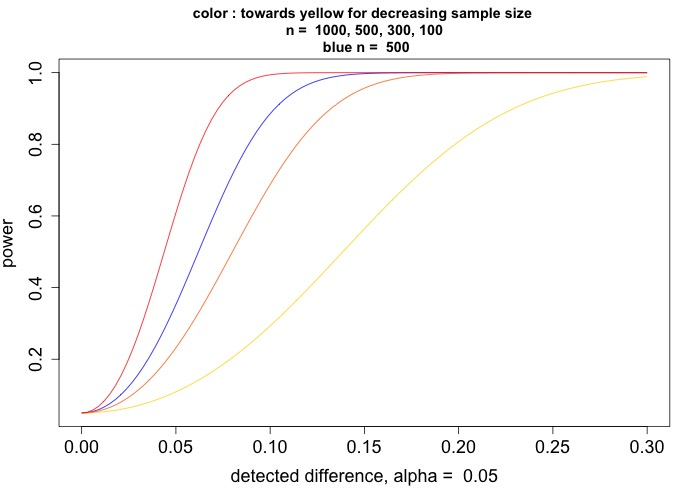
\includegraphics[scale=0.2]{plots/plot_power colore size 2.jpg}  
\end{minipage}
\caption{power as a function of effect size for different sample sizes}
\label{fig:power n}
\end{figure}
Considering the worst case, that is $\sigma_{D}\leq\sqrt{\frac{1}{2\cdot n}} $, from:
\begin{equation}
z_{1-\beta}+z_{1-\frac{\alpha}{2}} \simeq  d/\sigma_{D}\leq  \sqrt{2\cdot n}\cdot d
\end{equation}
it is possible to compute the sufficient sample size $n$ needed to detect a minimum effect size $d$ at $\alpha$ significance level and power $1-\beta$, as follows:\\
%defining effect size the value $d:= p_{1}- p_{2}$.
\begin{equation}
\textcolor{red}{n\geq \frac{1}{2}\cdot\left ( \frac{z_{1-\beta}+z_{1-\frac{\alpha}{2}} }{d}\right )^{2}}
\end{equation}\newline
It is worth to note that $n$ is inversely proportional to the square of the effect size. Fig.~\ref{fig:sample size beta} shows the sufficient sample size $n$ as a function of effect size at different powers at the given significance level $\alpha=0.05$.
\begin{figure}[h!]
\centering
\begin{minipage}{0.31\textwidth}
  \centering
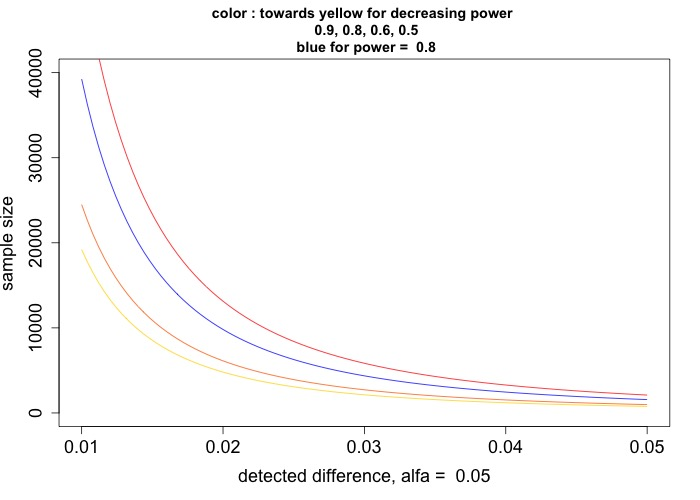
\includegraphics[scale=0.23]{plots/plot_samplesize VS effectsize_alfa_beta 1.jpg}  
\end{minipage}
\begin{minipage}{0.31\textwidth}
  \centering
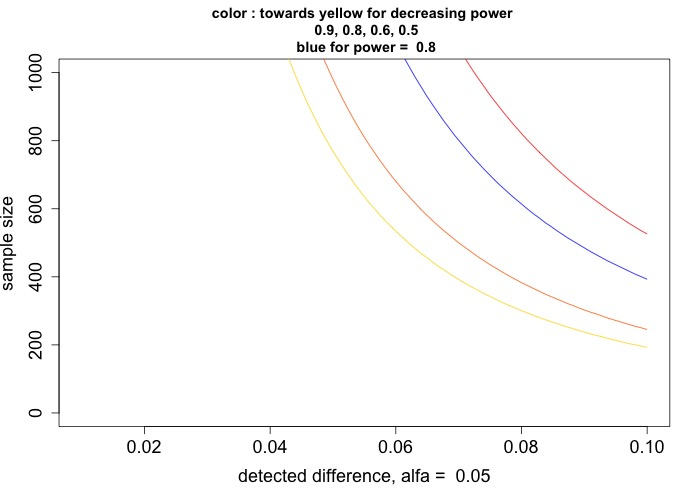
\includegraphics[scale=0.23]{plots/plot_samplesize VS effectsize_alfa_beta 2.jpg}  
\end{minipage}
\begin{minipage}{0.31\textwidth}
  \centering
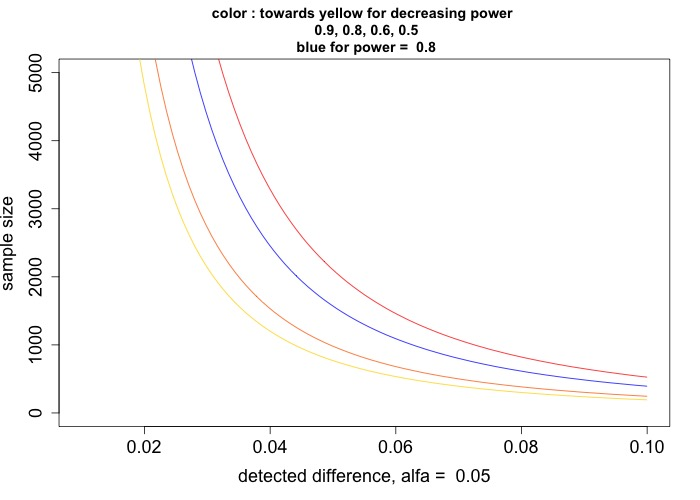
\includegraphics[scale=0.23]{plots/plot_samplesize VS effectsize_alfa_beta 3.jpg}  
\end{minipage}
\caption{$n$ as a function of effect size}
\label{fig:sample size alpha}
\end{figure}


 

\end{document}
